\documentclass[10pt,onecolumn,letterpaper]{article}

\usepackage{cvpr}
\usepackage{times}
\usepackage{epsfig}
\usepackage{graphicx}
\usepackage{amsmath}
\usepackage{amssymb}
\usepackage{listings}
\usepackage{amsthm}
\usepackage{mathtools}

\setlength{\parskip}{0.2cm}

\lstset{
basicstyle=\ttfamily,
frame=single
}


% Include other packages here, before hyperref.

% If you comment hyperref and then uncomment it, you should delete
% egpaper.aux before re-running latex.  (Or just hit 'q' on the first latex
% run, let it finish, and you should be clear).
\usepackage[breaklinks=true,bookmarks=false]{hyperref}

\cvprfinalcopy % *** Uncomment this line for the final submission

\def\cvprPaperID{****} % *** Enter the CVPR Paper ID here
\def\httilde{\mbox{\tt\raisebox{-.5ex}{\symbol{126}}}}

% Pages are numbered in submission mode, and unnumbered in camera-ready

%\ifcvprfinal\pagestyle{empty}\fi
\setcounter{page}{4321}

\begin{document}
%%%%%%%%% TITLE
\begin{titlepage}
                % \newgeometry{top=25mm,bottom=25mm,left=38mm,right=32mm}
                \setlength{\parindent}{0pt}
                \setlength{\parskip}{0pt}
                % \fontfamily{phv}\selectfont

                {
                                \Large
                                \raggedright
                                Imperial College London\\[17pt]
                                Department of Electrical and Electronic Engineering\\[17pt]
                                Final Year Project Report 2019\\[17pt]
                }

                \rule{\columnwidth}{3pt}
                \vfill
                \centering
                  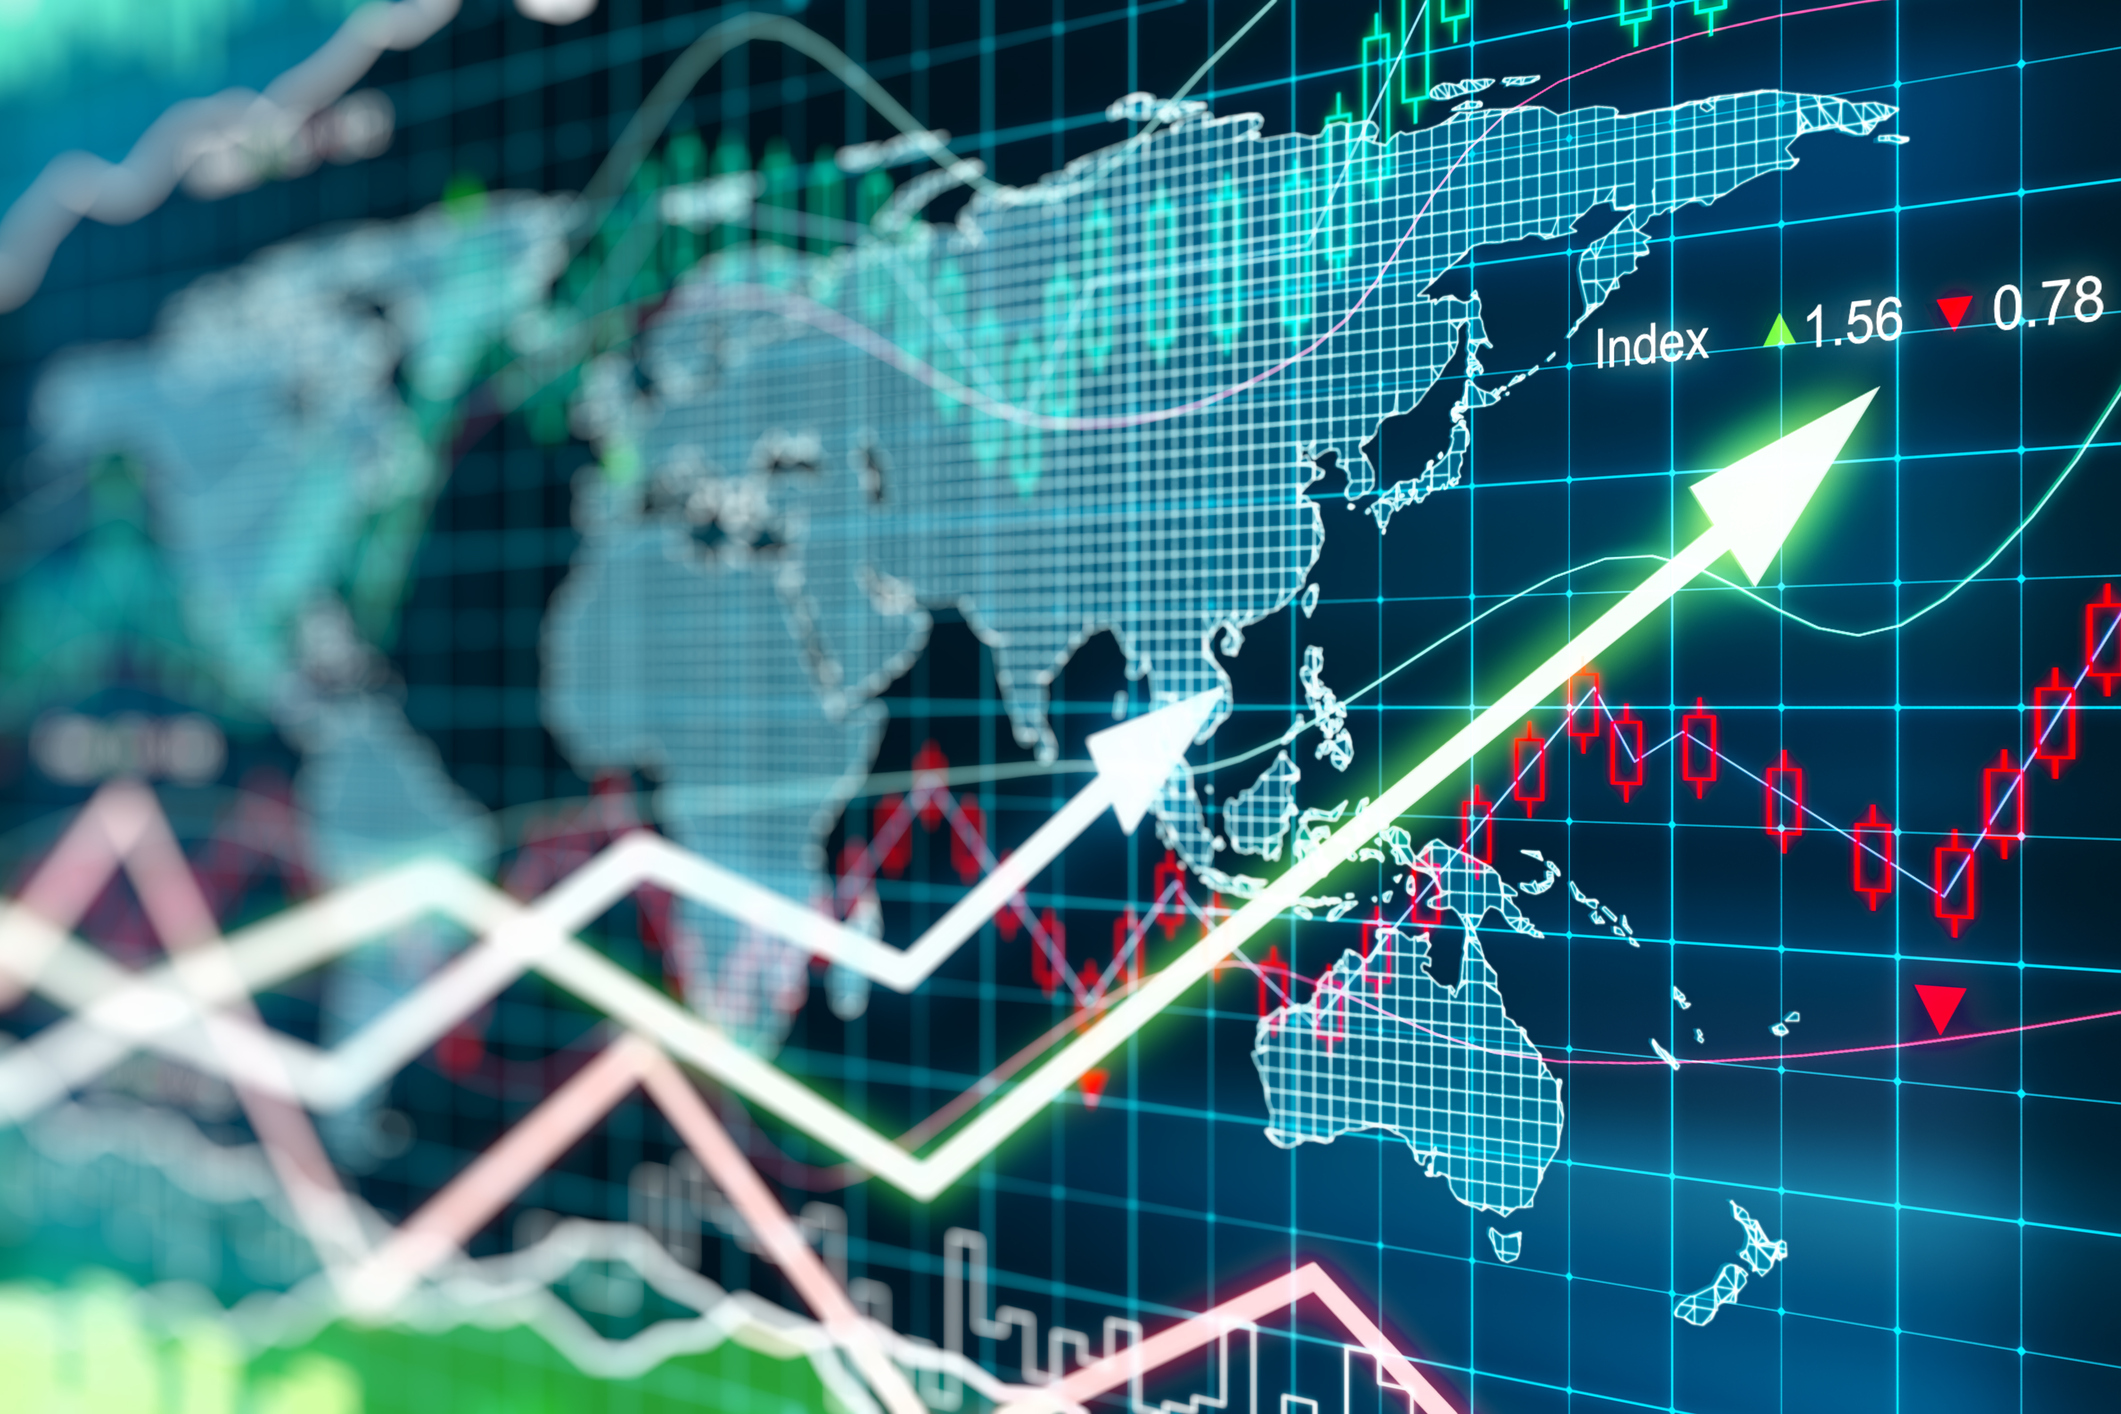
\includegraphics[width=0.7\columnwidth,height=60mm,keepaspectratio]{logo.png}
                \vfill
                \setlength{\tabcolsep}{0pt}
                \begin{tabular}{p{40mm}p{\dimexpr\columnwidth-40mm}}
                      	Project Title: & \textbf{Feature Engineering for Fundamental Factor Models} \\[12pt]
                       	Student: & \textbf{Tim Hung Wu} \\[12pt]
                        	CID: & \textbf{01195701} \\[12pt]
                	    	Course: & \textbf{EIE3} \\[12pt]
                        	Project Supervisor: & \textbf{Dr. Carlo Ciliberto} \\[12pt]
          		Second Marker: & \textbf{Professor Yiannis Demiris} \\[12pt]
                \end{tabular}
\end{titlepage}

%\thispagestyle{empty}

\begin{abstract}

This project explores the effectiveness of certain recurrent neural network architectures with long short-term memory units (LSTM RNNs) in the forecasting of stock prices for companies in the STOXX Europe 600 Industrial Goods and Services Index (SXNP). In particular, the project focused on attempting to identify whether certain attributes of a company’s fundamentals data, such as book value and annual sales, had significant influences on its stock price. The main emphasis of this project was to implement a complete tool that would provide all the functionalities required to take this machine learning problem from the initial raw dataset to a reasonable final forecast result. As such, the various processes required to develop a solution to a machine learning problem such as data preparation, network structuring, optimisation etc. were studied and analysed. A significant proportion of the project focused on processing the raw data into a suitable and effective format that could be used as the input of a Keras model. Additionally, by tuning various hyperparameters and experimenting with multiple loss functions and classifications methods, attempts were also made to optimize and improve the performance of the model. Finally, the stock weightings provided by the model were used to construct a portfolio to simulate a real world scenario. Its performance was then compared to the naïve diversification heuristic over a time period consisting of unseen test data. 
\end{abstract}

\section*{Acknowledgements}
A special thanks goes to Dr. Carlo Ciliberto of Imperial College London for taking the time to provide expertise about developing and designing a machine learning experiment. Additional thanks goes to Dr. Marco Bianchi and Michele Ragazzi of Giano Capital for providing the financial background knowledge to help bring this project to a real world application as well as their development team for providing the raw data. 

\newpage

\tableofcontents

\newpage

%%%%%%%%% BODY TEXT
\section{Introduction} 

\subsection{Project Motivation} \label{Project Motivation}

Public corporations are required to periodically report various fundamental financial data such as income statements and balance sheets. This is legally required in most countries for tax purposes and also provides key performance indicators for stakeholders and investors into the general financial health of a corporation. The owners of these companies are a mixture of the general public and ownership is fractionally divided via shares of a company's stock. These shares are able to be freely bought and sold and the process of valuing them has become of predominant interest to investors. Consequently, the expectation of how these valuations will deviate and change in the future is interesting as it provides the opportunity for financial gain by taking the profit through a difference in price. 

Academic research has demonstrated that some key factors of the reported financial data have historically had high correlation with the returns enjoyed by the stock of a company. An example of a popular methodology is analysing the asset turnover ratio ($sales/assets$), which approximately indicated the efficiency with which a company deploys its assets to generate sales. 

The process of automating the identification of features which are able to deliver profitable investment opportunities falls into the domain of  systematic factor investing. Increasingly, this has become more popularised because of the exponential technological improvements in data storage and computational power. Additionally, the digitalisation of data allows it to be more standardised and of higher quality, further lowering the limitations boundary for automation.  

\subsection{Problem Definition} \label{Problem Definition}

Using the SXNP dataset supplied by Giano Capital, this project aims to establish the key fundamentals that affect the returns of a company's stock price. This is achieved by developing algorithms that can assist in predicting the future prices of the stock. The algorithms utilise several inputs such as book value, sales and profit of the specified company to train and learn a function that correlates with the price. The performance is then benchmarked against an industry standard to see if the algorithms have achieved any outperformance compared to traditional models. This problem falls in the scope of machine learning, which has been frequently used to produce solutions in data-driven problems in recent times. Focus will be directed at RNNs with LSTM units. We choose well established and tested techniques used in literature to extract features from the dataset and attempt to learn patterns in the data. We will then tune the hyperparameters to optimise the model, and evaluate its potential performance in a pseudo-generated real world application. 

\subsubsection{Intended Deliverables} \label{Intended Deliverables}
\begin{itemize}
	\item A cleaned dataset capable of being trained on. 
	\item A piece of software that implements a predictive model. 
	\item Analysis into the performance of the model.
	\item Understanding of prior research in the area and how to design a machine learning experiment. 
	\item A report and poster summarising the project and its experimental results.
\end{itemize}

\subsection{Importance in Industry} 

Outperformance, defined by generating excess returns above the market average, is termed as alpha ($\alpha$) in the financial industry. This metric is widely used to assess and compare the abilities of actively managed funds. The process from which alpha is generated is termed "signal generation" and determines when a security, such as a stock, should be bought or sold. However, as more people utilise a certain signal, it becomes weaker as it, by definition, tends towards becoming part of the market average. The objective then evolves to be consistently producing new, stronger signals. As mentioned in section \ref{History of Investing Methodologies}, there are various methodologies people use to generate signals. Although there is no limit to how complex a signals can theoretically be, people tend to focus on just a handful of parameters for ease-of-use and understanding. This begs the question of whether a machine learning model, with increased numbers of inputs, are able to assist in developing or even create complex methodologies that result in strong signals.  

As such, this project is of interest to money managers as a means from which to develop alternative and new solutions to the problem of generating new signals to produce alpha. Additionally, the consequence of being able to produce improved returns are ultimately handed to the investors. This project focuses particularly on the fundamental components of companies, which tends to be in the scope of long term investment. The investors in these areas often include institutional clients such as pension funds meaning that these potential improvements are eventually passed down to working individuals, who do not possess the ability to generate this income on their own for their future retirements.  

\subsection{Software Usage} 

Python will be the language used for software development given the extensive number of libraries that offer the opportunity for the fast development required for the project. The key packages that will be used are Pandas and Keras, which are data manipulation and machine learning tools respectively. Correctness of the code is a necessity whereas performance is treated as a luxury. The report will be written in LaTeX. 

All software development will be within the student's personal Google drive, with external view access granted to only those that are necessary. A web based environment, Jupyter Notebooks\cite{jupyter_notebook}, will be used in order to develop a clear and structured front end document that can be easily used and interacted with by users. Consequently, the ipynb file format will be used for the source. Data is stored as csv files. 

Cloud services will be used for the computational power and elements of data storage. Google Colaboratory offers good support for the Notebook and has previously been used as part of the EE3-25 Deep Learning module and so has a low barrier to entry. Given the fairly small size of the dataset (at approximately 300MB), the required computation power required is estimated to be well below the maximum threshold of the environment. 

\subsection{Report Structure} \label{Report Structure}

This report begins with a background outline to provide more colour into the problem by highlighting historical approaches. It will then establish a benchmark evaluation metric for the problem to objectively measure performances. This will be followed by a detailed discussion of the design processes of our approaches. Afterwards, the challenges of the actual implementation of the various models will be discussed, with comments about how their designs were modified from the initial specification to build the final solution. Finally, we will test and analyse the systems against our self-developed metrics, noting down all the key discoveries and findings learned throughout the project before concluding the direction in which the project could be further developed in the future. 

\newpage

\section{Background}

\subsection{History of Investing Methodologies}  \label{History of Investing Methodologies}
The fundamental question that the project is attempting to answer is what drives stock price and their underlying returns. This has been tackled through a whole range of varied approaches ever since shares of stock were first offered to general public in the early 1600s by the Dutch East India Company\cite{Rouwenhorst}. In 1934, Benjamin Graham et al. introduced the first formal framework for security analysis\cite{Graham}. In his book, he describes the differences of market behaviour in the short and long run. Graham observed that fear, greed and emotions were the main drivers of short-term market fluctuations which can cause discrepancies between the pricing and true value of a company's stock. However, over long periods of time, Graham perceived that a company's fundamentals are the critical price driver, which causes the market pricing of the stock to converge with its true value. These observations formed one of the first formal distinctions between speculation and investment.

The first formal model\cite{Treynor} of analysing stock returns was introduced by Treynor et al. in the 1960s. It was called the Capital Asset Pricing Model (CAPM) and focused on the idiosyncratic and systematic risk of an asset relative to the market. The formula for pricing a security is as follow: $E(R_{i}) = R_{f} + \beta_{i}(E(R_{m}) - R_{f}) $ where $E(R_{i})$ is the expected return of investment, $R_{f}$ is the risk free rate, $\beta_{i}$ is the beta of the investment, $E(R_{m})$ is the expected return of the market. In other words, the expected return of a stock can be viewed as a function of its correlation to the market. 

An alternative theory\cite{Ross} about what drivers stock returns was later proposed by Ross in 1976. Arbitrage pricing theory (APT) postures that the expected return of a financial asset can be modelled as a function of various macroeconomic factors. Ross is often accredited with popularising the term "multi-factor models." Crucially, APT performed better than CAPM because it did not explicitly state a set of fixed factors. Instead, factors were assumed to vary across markets and differ over time. The challenge then boiled down to identifying the factors that best describe a specific region at a point in time. 

Arguably, the most utilised factors for analysis are fundamental factors, which capture the characteristics of a stock. One of the most well known attempts in this space was derived from Fama and French in the early 1990s. Their model\cite{Fama} explained US equity market returns from three factors: size, value and correlation as mentioned in the CAPM model. The fundamental objective of factor investing is to achieve enhanced diversification, above-market returns and reduced risk exposure. The numbers of quantifiable factors are vast but typically, are broken down into five predominant categories: 

\begin{itemize}
	\item Value: The stocks usually trade at low prices relative to their fundamental indicators. These are identified via indicators which are typically ratios such as $\frac{bookvalue}{price}$, $\frac{earnings}{price}$ or $\frac{dividend}{price}$. When these ratios are significantly higher than the average company within the same sector, the company can be classified as having value stock. It should be noted that average ratios vary between sectors and so cross-industry comparisons cannot be made. 
	\item Size: Eun et al. demonstrate in their research\cite{Eun} that small capitalisation stocks tend to exhibit statistically significant returns and diversification than large capitalisation stocks when allocated in international funds. Capitalisation is defined as $capitalisation = no.share * share price$. Small-caps are defined to range from valuations of \$300 million to \$2 billion. 
	\item Momentum: Stocks that have exhibited outperformance in the past tend to follow the same trend in the future. Strategies involving momentum often involve analysing, ranking and allocating to the highest returning stocks within a specified time frame such as one year or three years. 
	\item Quality: These stocks are typically categorised by certain fundamentals such as low debt, average earnings with low standard deviation i.e. high stability and consistent asset growth i.e. the derivative of book value with respect to time is fairly uniform. Common financial metrics used to help identify this include the return on equity ($ROE = \frac{NetIncome}{ShareholderEquity}$) or the debt-to-equity ratio ($\frac{D}{E} = \frac{Total Liabilities}{Total Shareholder Equity}$.)
	\item Volatility: Empirical research by UBS\cite{Merz} suggests that low volatility stocks earn greater risk-adjusted returns than other stocks, with particular outperformance during stressed market environments. These are often ranked and selected by measuring the standard deviation of a stock's return. 
\end{itemize}

\subsection{Long Short-Term Memory Networks} \label{lstm}

\subsubsection{Overview} 

LSTM networks are derived from RNN models, which were first introduced into literature\cite{Rumelhart} in 1986 by Rumelhart et al. Rumelhart was a psychologist by training and the initial objective was to provide an alternative framework for understanding cognitive perception. The fundamental problem was to highlight that human perception and learning were formed through temporal experience and so a model was required that could process and partially remember sequential data. Rumelhart mathematically modelled this as $h_{t} = f_{W} (h_{t-1}, x{t})$ where $h$ is the state, $x$ is the input with respect to the time interval $t$ and $f$ is a function generated by the parameters $W$ as determined by the configuration of the LSTM cell. This was in contrast with more traditional neural networks, such as the multilayer perceptron (MLP), are structured in a feedforward fashion that do not share weights, meaning that there are no cycles formed within the nodes. 

\begin{figure}[!hbt!]
\centering
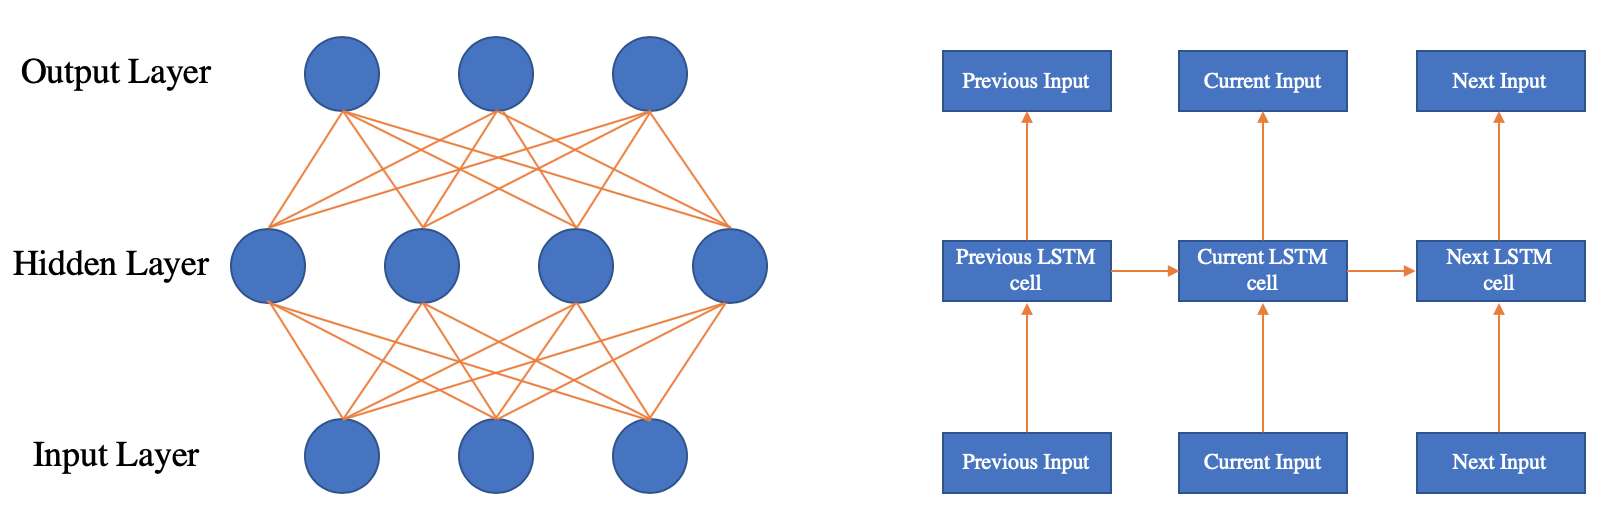
\includegraphics[width=17.5cm]{mlp_rnn_comparison.png}
\caption{A classical MLP (LHS) simply generates an output with respect to its input whereas in the RNN (RHS), the output is governed by the input and previous input.}
\end{figure}

The use cases of RNNs have since expanded to multiple, practical domains that heavily use sequential data, such as text generation, visual recognition and time series prediction. Part of the advantages offered by RNNs is the various topologies in which it can be structured. The most vanilla case is with a direct one-to-one mapping. However they often change to many-to-one, many-to-many or one-to-many to suit the task at hand. 

\begin{figure}[!hbt!]
\centering
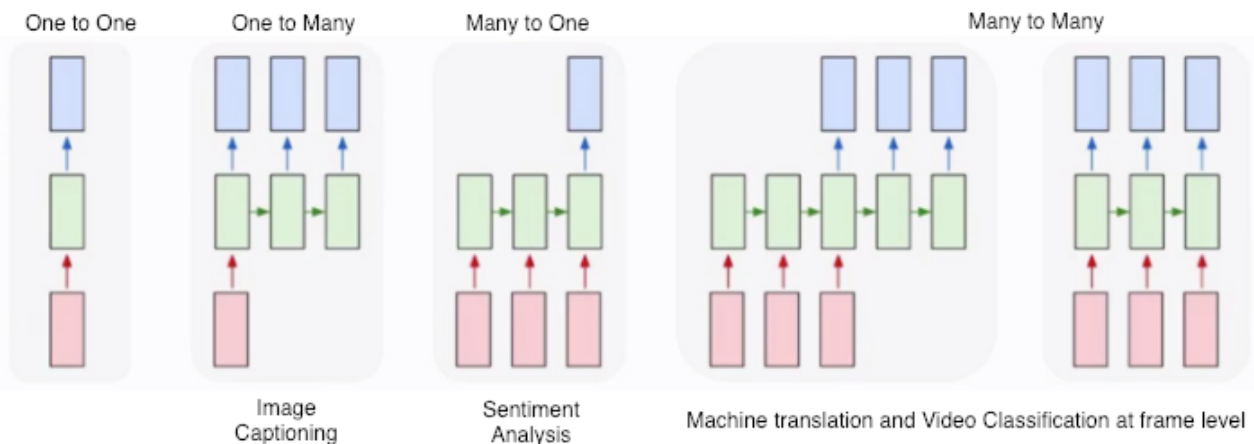
\includegraphics[width=14.5cm]{rnn_topologies.png}
\caption{Numerous varying topologies for specific sequential data tasks.}
\end{figure}

An issue with RNNs stem from the inherent property of operating with a sequential nature. The time difference between multiple cell often causes issues during backpropogation involving repeated multiplication of the gradient signal. This means that if the partial derivatives of the error gradient are either too large or small, they can explode or vanish respectively during the procedure. Exploding gradients cause the learning to diverge whereas vanishing ones can cause the learning rate to become very slow and eventually stop, as it tends to 0.
 
\begin{proof}\renewcommand{\qedsymbol}{}
Let $x, y, h,  \theta, f $ be the input, output, hidden state, weights and basis function respectively: (Bengio et al.)
	\begin{align*}
    	h_{t} &=  \theta f(h_{t-1}+\theta_{x}x_{t})\\
    	y_{t} &= \theta_{y} f(h_{t}) \\
    	\shortintertext{The loss function is then:} 
    	\frac{\partial E}{\partial \theta} &= \sum_{t=1}^{S} \frac{\partial E_{t}}{\partial \theta} \\
  	\frac{\partial E_{t}}{\partial \theta} &= \sum_{k=1}^{t} \frac{\partial E_{t}}{\partial y_{t}} \frac{\partial  y_{t}}{\partial h_{t}} \frac{\partial h_{t}}{\partial h_{k}} \frac{\partial h_{k}}{\partial \theta} \tag{where $k$ are the layers before time $t$} \\
	\shortintertext{The third term of the chain, $\frac{\partial h_{t}}{\partial h_{k}}$, is a product of Jacobians such that:} 
	\frac{\partial h_{t}}{\partial h_{k}} &= \prod_{i = k+1}^{t} \frac{\partial h_{i}}{\partial h_{i-1}} = \prod_{i = k+1}^{t} \theta^{T}  diag(f'(h_{i-1})) \\
	||\frac{\partial h_{i}}{\partial h_{i-1}}|| & \leq ||\theta^{T}|| ||diag(f'(h_{i-1}))|| \leq \gamma_{\theta}\gamma_{f} \tag{ where $\gamma$ are the constants that upper bound the two terms} \\
	||\frac{\partial h_{i}}{\partial h_{i-1}}|| & \leq  (\gamma_{\theta}\gamma_{f})^{t-k} &&\qedhere \\
 	\end{align*}
\end{proof}
\vskip -0.5cm
This implies that if $\gamma_{\theta}\gamma_{f} > 1$ or very small, the gradient will explode or vanish given a large $t-k$. LSTMs were first introduced by Hockreiter et al.\cite{Hockreiter} in 1997 and were effective at correcting the vanishing gradient problem. LSTMs use gating, also known as component-wise multiplication, which allows for more control over the gradient flow and thus enables better preservation of long term dependencies. Three gates exist in the LSTM cell forget, input and update, which are mathematically defined as following: 

\begin{gather*}
 	\text{Forget gate}: f_{t} =  \sigma(W_{f}(h_{t-1},x_{t}) + b_{f}) \\
	\text{Input gate}: i_{t} =  \sigma(W_{i}(h_{t-1},x_{t}) + b_{i}) \\
	\text{Update gate}: u_{t} =  \sigma(W_{u}(h_{t-1},x_{t}) + b_{u}) \\
	\shortintertext{As explained by Olah\cite{Olah}, the forget gate controls the fraction of how much of the previous cell's information should be retained. Next, a decision needs to be made about what new information should be stored in the current cell. This is achieved by the input gate. Additional to this, a candidate cell, $\tilde{C}$, is produced and scaled appropriately with a $tanh$ layer. By combining these two it is possible to create an update to the state.} 
	\tilde{C_{t}} = tanh(W_{C}(h_{t-1},x_{t}) + b_{C}) \\
	C_{t} = (f_{t} \times C_{t-1}) + (i_{t} \times \tilde{C_{t}})
	\shortintertext{The block output will then be a filtered version of our newly updated cell state, with the filter being the update gate. The sigmoid layer in the update gate decides what parts of the cell state will be output.} 
	y_{t} = u_{t} \times tanh(C_{t})
\end{gather*}

\begin{figure}[!hbt!]
\centering
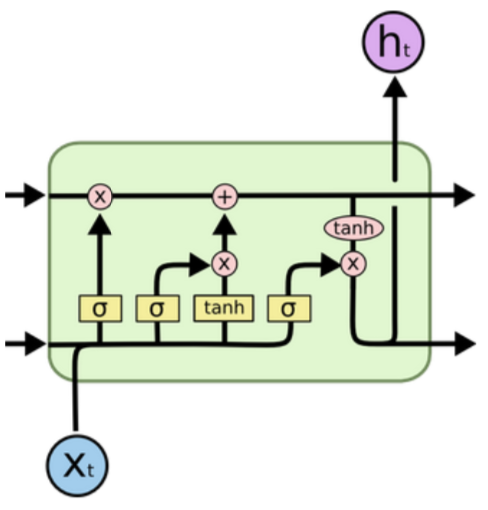
\includegraphics[width=4.5cm]{lstm_unit.png}
\caption{Breakdown of a LSTM cell depicting the input, forget and update gates.}
\end{figure}

\subsubsection{Loss Functions} \label{loss functions}

The loss function is important in the feedback mechanism of general neural networks and vary given the task at hand. They typically fall into two categories depending on the problem itself: classification and regression. These domains treat discrete and continuous value labelling problems. 

For regression problems, two of the most common loss functions used are mean squared error (MSE) and mean absolute error (MAE). Mathematically, there are defined as following: $MSE = \frac{1}{N}\sum_{i = 1}^{N}(x_{i}-y_{i})^2$, $MAE = \frac{1}{N}\sum_{i = 1}^{N}|x_{i}-y_{i}|$. The difference in the behaviour of the loss functions can be observed with large errors, with MSE putting much more emphasis on learning and correcting from those data points. Interestingly, Janocha et al.\cite{Janocha} suggested that these loss functions also perform surprisingly well in deep net classification objectives as a means of providing a probabilistic interpretation in terms of expected misclassification.

A popular example of a classification problem is the a binary classifier. These take input data and assign one of two possible output values. An example would be the binary cross-entropy loss function, expressed as $\frac{1}{N}\sum_{i = 1}^{N}log(p(y_{i}))-(1-y_{i})(log(p(1-y_{i})))$ where $y_{i}$ is the target label. 

\subsubsection{Cross Validation} \label{cross validation}

An issue with LSTM networks arises when using classical cross validation methods. K-fold cross validation involves dividing the data into $k$ folds before assigning the initial fold as the test data and the rest as the training data. After each iteration of training, the test data assignment is then incremented until its position has permeated through all of the positions. However, with sequential data, this method causes disjoints in the training data since training for fold $n+1$ will be involve information from $n-1$ rather than $n$. In 2015, Bergmeir et al. introduced a new method\cite{Bergmeir} to handle cross validation for time-series data. Their system involved a forward chaining concept such that training data is never interrupted. Although it resolves the issue, the generalisation error is then affected by the change in training data size. Below is a heuristic for the method: 

\begin{itemize}
 	\item Divide the data into $k$ folds. 
	\item 1st iteration: Training on fold 1. Testing on fold 2.
	\item 2nd iteration: Training on fold 1, 2. Testing on fold 3. 
	\item Repeated to $k-1$th iteration: Training on fold 1, 2 ... $k-1$. Testing on fold $k$ (last fold). 
\end{itemize}

An alternative solution\cite{Racine} was also proposed by Racine. He observed that what was truly needed is independence between the training and test data sets. This can be approximated by removing adjacent folds which will be highly dependent on and correlate with the test fold. This needs to be performed on both sides of the test fold as dependence is symmetric when moving forwards and backwards in time. This approach is known as $hv$ cross validation where $v$ is the test fold and $h$ are the number of observations on each side of the test fold. Below is a heuristic of the method:

\begin{itemize}
 	\item Divide the data into $k$ folds. Assume $h = 1$ 
	\item 1st iteration: Testing on fold 1. Fold 2 is discard. Training occurs on the rest of the folds. 
	\item 2nd iteration: Training on fold 2.  Folds 1 and 3 are discarded. Training occurs on the rest of the folds. 
	\item 3rd iteration: Training on fold 3.  Folds 2 and 4 are discarded. Training occurs on the rest of the folds. 
	\item Repeated to $k$th iteration Testing on fold $k$ (last fold). Fold $k-1$ is discard. Training occurs on the rest of the folds. 
\end{itemize}

This does not introduce the generalisation error as in Bergmeir's method. However, it is more complex to measure the $h$ required to approximate a good independence and there is still a consistent inefficiency in data usage given the discarded folds are not trained or tested with. This efficiency is only better than Bergmeir when $h \leq 2\times(\frac{k^{2}}{2}) = k^{2}$. Both methods will be used during the project to determine which one is optimal.

\subsubsection{Applications} 

An exciting application of LSTM networks can be found in one of Google Deepmind's project called Deep Recurrent Attentive Writer (DRAW). In their paper\cite{Gregor}, Gregor et al. outline the architecture for a network capable of image generation. They use a variational autoencoder (VAE) as the generative model. This encodes a raw image into a lower dimensionality vector, which forces the encoder to learn the features of the image. LSTMs and attention mechanisms are then used to iterate this encode-decode procedure. This network was used to generate digits after being trained on the Modified National Institute of Standards and Technology (MNIST) database. 

\begin{figure}[!hbt!]
\centering
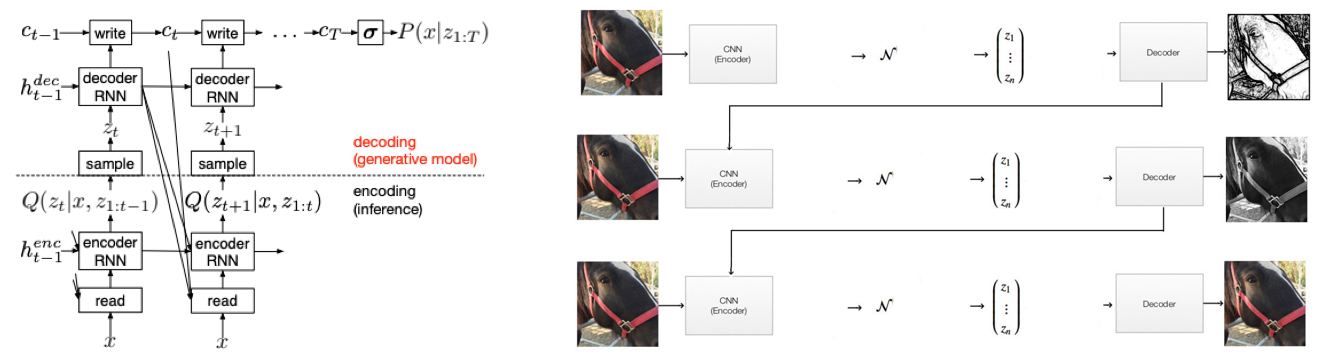
\includegraphics[width=14.5cm]{draw_network.png}
\caption{LHS: DRAW network from Google Deepmind, featuring an attention mechanism formed by an encoding and decoding RNN (with the LSTM architecture). RHS: Simulation of how each iteration improves on the previous when using the network.}
\end{figure}

\begin{figure}[!hbt!]
\centering
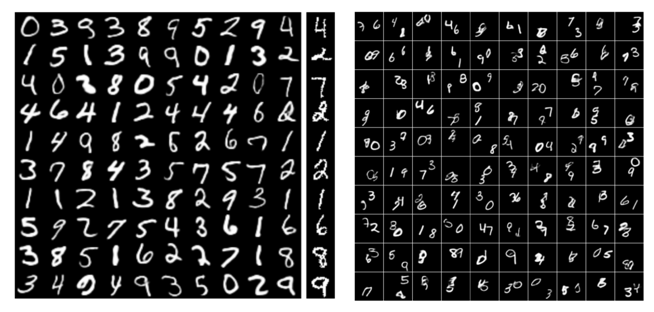
\includegraphics[width=12.5cm]{draw_results.png}
\caption{LHS: Single digits generated from the MNIST database, with the right-most column depicting original images from the database. RHS: DRAW's attempts at generating double digit values.}
\end{figure}

Groundbreaking work can often be produced and found in competitions. The primarily example for time-series datasets was the M4 competition held in June by Makridakis of the University of Nicosia. This was the forth competition of a series which focussed on forecasting for 100,000 time-series datasets, spanning different time intervals and domains. A key objective of the task was to evaluate the performance of machine learning models compared to other statistical methodologies. Makridakis et al.\cite{Makridakis} published their findings after the competition. Below are a few of their major findings in the report:

\begin{itemize}
	\item Combination of methods performed well in the M4 competition - 12 of the 17 most accurate methods were combinations of mostly statistical approaches.
	\item The best performing approach utilised both statistical and ML features. This method produced the most accurate forecasts as well as the most precise Prediction Intervals and was submitted by Smyl, Data Scientist at Uber Technologies. According to competition error metric, Symmetric Mean Absolute Percent Error (sMAPE), it was close to 10\% more accurate than the Combination benchmark of the Competition. It is noted that in the M3 Competition (Makridakis \& Hibon, 2000) the best method was 4\% more accurate than the same benchmark.
	\item The second most accurate method was a combination of seven statistical methods and one ML one submitted jointly by Spain’s University of A Coruña and Australia’s Monash University.
	\item The six pure ML methods submitted performed poorly, none of them being more accurate than the benchmark.
\end{itemize}



\subsection{Review of Machine Learning Research in Investing}  \label{ML_research}

Machine learning research in finance applications often span two domains; applied research in financial firms often has a more pragmatic approach and a more theoretical approach is usually observed in academic institutions. Man Group, a quantitative investment management firm, have been conducting research\cite{Man_Group} within the machine learning domain for decades but have only in the past five years begun actively applying models in a live environment. This is because there have only been enough developments recently in infrastructural support to help scale these models onto a production level. They separate their approaches into two major categories:
\begin{itemize}
	\item Deep Learning: Models using artificial neural networks which are trained on large data sets to identify special features. The traditional application of these techniques stem from areas such as image recognition but can also be used to learn predictive patterns in financial datasets. 
	\item Natural Language Processing: This mainly involves the automation of analysing written reports, such as a company's financial statements or a shareholder letter. Techniques involve assigning numerical values that measure the sentiment of these reports, which are often correlated with the price. This provides an unbiased and deterministic method for evaluating stocks. 
\end{itemize}
The model used in the project falls under the deep learning categorisation and is specified in section \ref{lstm}. A few questions come to surface regarding the technical challenges of the implementation. Some are listed below and answered by various approaches recommended in numerous papers: 
\begin{itemize}
	\item Normalisation: Standardising the features of a model is often important because there is a need to compare measurements which have different units. 
	\item Missing Inputs: A way of handling incomplete datasets is needed. Methodologies often fall into the two categories of either regenerating or masking the missing values. 
	\item Encoding Additional Information: Adding human derived formulas such as $\frac{sales}{assets}$ can be seen as generating human bias or assisting the model with classification depending on perspective. 
	\item Cross Validation (Section \ref{cross validation}): A problem with time series structures is the autocorrelation of data points. This means that typically cross validation methods such as leave-one-out introduce issues by missing information in the series and leaking information from the future. 
\end{itemize}
One of the earliest published papers\cite{Ahmadi} regarding the subject matter was written by Ahmadi in 1990. It was primarily focused on sourcing an alternate approach to generating a more comprehensive system to analyse factors in the APT model. This was done as following: Given a $N\times T$ matrix, $r_{N,T}$ is defined as the return of asset $N$ at time period $T$. For this matrix, there is a smaller one of $K\times T$, where $f_{K,T}$ represents the $K$th factor score for time period $T$. Thus, the return of a given asset is: 
$R_{N} = E_{N} + b_{N,1}F_{1} ... + b_{N,K}F_{K} + e_{N}$ where $E_{N}$ is the expected return, $e_{N}$ is a random zero mean error term and  $b_{N,K}$ are the estimated coefficients for each factor. Using the coefficient estimates, it is possible to employ another variable, $\lambda$, to determine whether it is statistically significant and thus whether the factor is significant. This is done with the following equation: $E_{N} = \lambda_{0} + b_{N,1}\lambda_{1} ... + b_{N,K}\lambda_{K}$.

The problem Ahmadi wanted to resolve was the heavy dependency on the sample that factor analysis relied on. There was a significant chance that, given 42 groups of 30 stocks each, different significant factors would be discovered in each group. He therefore employed a neural network so that, rather than optimising and identifying the statistically significance in each feature individually, the patterns stem from analysing the whole vector space. Ahmadi provides some details about the network, highlighting that the inputs used were the unemployment and inflation rates, rate of returns of assets, rate of change in the stock market and the change in gross national product (GNP). He also specifies that the inputs were normalised, two hidden layers offered the best optimal performance and the learning plateaued after 5000 iterations. 

As machine learning research became more formalised, the structure of experimentation was more defined. Kim published a paper\cite{Kim} in 2003, focused on understanding how support vector machines (SVMs) fared at predicting the Korea Composite Stock Price Index (KOSPI). Performance, $P$, was measured using the following equation: 

\begin{gather*}
 	P = \frac{1}{m} \sum_{i=1}^{m} R_{i} \tag{i = 1, 2, ... m} \\
	\shortintertext{where $R_{i}$ is the prediction result for the $i$th trading day as defined by:} 
\end{gather*}

\vskip -1cm
\[R_{i} = 
\begin{cases}
	1,& \text{if } f(x) = y\\
	0,& \text{otherwise}
\end{cases}
\]

where $f(x)$ is the prediction and $y$ is the actual value.

He tested the structure with both the polynomial and Gaussian radial basis functions for the kernel. Most importantly, he benchmarked the performance against two other models: a three layered backpropogation network (BP) and case based reasoning model (CBR) using nearest neighbour. However, there are no specific details about the architectures of these models. 

\begin{figure}[!hbt!]
\centering
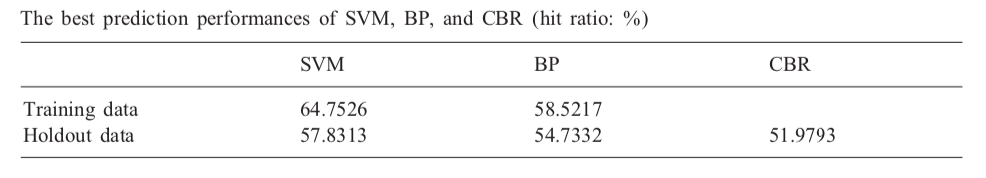
\includegraphics[width=14.5cm]{Kim_results.png}
\caption{Kim's results of SVM compared to BP and CBR.}
\end{figure}
 
An interesting alternative approach\cite{Alberg} is demonstrated by Alberg et al. who tackles the problem from a different perspective and adapts the classical problem from predicting prices to predicting how the fundamentals of a company will change. These predictions could then be used in turn to indirectly predict the price at that future time point. Alberg then backtested this idea, accessing existing fundamentals data as the 'future predicted fundamental', equating its price and evaluating the performance of the model. The paper goes into great depth about the set up of the experiment. A key area of interest is the methodology used to establish the binary output classifier: 

\[f(x)= 
\begin{cases}
	1,& \text{if } x > \frac{n+1}{n}th\text{ term}\\
    	-1,& \text{if } x < \frac{n+1}{n}th\text{ term}
\end{cases}
\]

\begin{figure}[!hbt!]
\centering
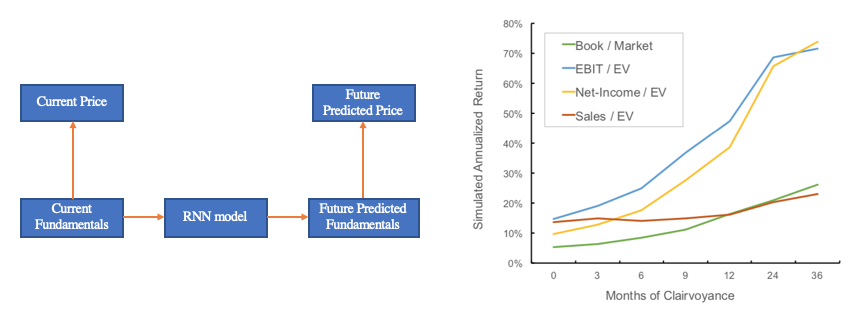
\includegraphics[width=14.5cm]{alberg_intro.png}
\caption{(LHS) The overview of how the model functions. (RHS) Backtesting results from Alberg with various factor models between 2000-2016. Clairvoyance x-axis equates to the time period difference between the current and future time in the model. }
\end{figure}

Rather than predicting the prices directly, which could rely on a multitude of factors outside just fundamental data, the model is structured so that it is interested in learning about what makes a company outperform the median return. A weakness of this classifier is that, in economic downturns, the median return could still be negative and so the model is not learning what fundamentally drives 'good' returns in an absolute sense. It also does not predict the degree to which the chosen stocks will outperform. However, this is in interesting structure for this project given the relative nature of the evaluation metric selected as mentioned in section \ref{benchmark}.

Additionally, normalisation of the inputs is carried out with two methods. The first involves ranking the performance of stocks against a certain ratio, such as $\frac{Book Value}{Market Capitalisation}$. The percentiles of their rankings are then inputted alongside the raw scores in order to produce a more comparable set of features between various stocks. The second involves transforming all data points into a specified domain for ease-of-use to the learning algorithm whilst maintaining the same relative fundamental values between companies. Alberg achieves this by dividing the input feature by the L2 norm of all the features ($x_{i} \rightarrow \frac{x_{i}}{||x||}$). This is in contrast with two of the more popular methods of normalisation: z-score ($x_{i} \rightarrow \frac{x_{i}-\mu_{x}}{\sigma_{x}}$) where $\mu$ and $\sigma$ are the mean and standard deviation and min-max scaling ($x_{i} \rightarrow \frac{x_{i}-x_{min}}{x_{max}-x_{i}})$.

Finally, in 2019, a summary of the literature\cite{Henrique} that had been written about financial prediction applications using machine learning was produced by Henrique et al. They constructed a table comprehensively detailing the various attributes and methods used in the papers they reviewed. This provides a very general overview into how the academic field is generally designing experiments for this problem domain.

\begin{itemize}
	\item Assets Evaluated: Typically stocks or indices. These fall into the same region as the problem tackled by this project. Interestingly, many index models were focused on predicting the prices of the index itself whereas stocks typically offered more dynamic evaluation metrics such as selecting good stocks and calculating their returns.
	\item Predictive Variables: Predominately technical analysis or prices, with a few fundamentals and one text and news. It is understandable that most models which predict price use technical analysis indicators given that the perceived relationship between these is fairly strong. Technical analysis was designed for price analysis whereas fundamental data looks at the valuation of stocks, which is a slightly different task. However, this project focuses on a long term investment horizon and so is hoped that fundamental features will be more significant in this time domain. The text and news cases were used to analyse sentiment, which often affects price on a very short time horizon.
	\item Output Prediction: Mainly prices, return or direction, with a couple targeting volatility. Price and returns are the ideal goal but it is interesting to see that a significant number of models use alternate methodologies. Both direction and volatility offer a less demanding output objectives and so could achieve better results overall if trained correctly. This project will analyse a variety of output predictors and compare their performances.
	\item Methodology: Mostly neural networks, with some SVMs and fuzzy logic. This project uses a RNN with LSTM units and so falls under the set of neural networks. The objective is to explore how LSTM models fare in a different domain, given their primary applications being in image, audio and text generation/recognition.
	\item Performance Measure: A mixture of return, Sharpe ratio, mean absolute error (MAE) and mean squared error (MSE). MAE and MSE are generally used when classifying the test error of a price prediction. However, the project aims to deliver a real world grounding and so metrics such as Sharpe ratio will be used during the final evaluation. It is very likely that MAE and MSE will be analysed during the experimentation stages. 
\end{itemize}

%-------------------------------------------------------------------------
\newpage

\section{Requirements Capture} 

The key objective for the project is to deliver a tool that will assist in answering the fundamental problem of whether it is possible to predict price changes in stocks based on the fundamental's data of a company. This primary objective is then divided into sub-sectional physical deliverables, as briefly mentioned in section \ref{Intended Deliverables}. Fallback plans were established for each deliverable to prioritise certain essential functionalities if problems in software development and debugging cause significant time delays. 

\subsection{Tasks}
\begin{enumerate}
	\item Data Preprocessing: Using methods that have been researched and understood, the datasets supplied by Giano Capital will be cleaned and formatted in an appropriate fashion for use as the inputs of the LSTM model. This is a vital element of the project and it can be argued that the quality of model performance is critically dependent on this deliverable. However, it is important to observe the schedule as this is the initial deliverable and going overtime would put the other components in jeopardy. In a worst case scenario, priorities will be made to certain fundamentals that are theorised to be the most important and the others discarded to reduce workload.
	 \item Building and Testing Benchmark: The design for a suitable industry-standard benchmark is mentioned in section \ref{benchmark}. Going forwards, the objective will be to build the tools necessary to compare the benchmark with the output data from the model. Similar to the fallback plan in Data Preprocessing, efforts will be solely concentrated on the key benchmark criteria (the most important being absolute returns) if there are heavy time constraints. 
	\item Implementing and Testing Model Architecture: Official documentation about the Keras API alongside example notebooks from the EE3-25 Deep Learning module will provide the basis for developing a well structured and coherent architecture. Initially, a simplistic baseline model will be constructed and tested in order to provide a fundamental level from which to develop a better and more sophisticated model. Parameters will be experimented with by applying similar logic to the research methods discussed in section \ref{ML_research}. If time constraints become an issue, a simpler model will be developed and tested instead, with the baseline model being used in the absolute worst case scenario. 
	\item Integration Testing and Debugging: The prior three deliverables form components of the system and so will need to be tested when combined to see if the behaviour and results are as intended. This deliverable is flexible as testing can be performed to a wide degree of formality. A rigorous framework will require the construction of test datasets and their intended outputs, accounting for all edge cases that may occur. Consequently, significant time may need to be spend debugging and restructuring the codebase to account for these edge cases. The primary focus is for the development of a robust rather than an entirely correct system. The fallback plan is therefore to solely focus on accounting for errors that may occur in the Giano dataset as ultimately, this is what the model will use to perform analysis. 
	\item Hyperparameter Optimisation: To improve the performance of the model with respect to the benchmark, various modifications can be applied to areas of the algorithm such as the training method, network depth, learning rate optimisers etc. A significant proportion of time has been allocated to this since it involves the lengthy process of retesting and reevaluating the results and performance given every adjustment made. This final deliverable is arbitrarily long, given the fact that analysis of components can be inexhaustibly extensive and so it will be flexible in the sense that as much experimentation will be performed as allowed for by time. 
\end{enumerate}

\newpage

\section{Design and Analysis}
Give a good high-level overview of your design.

Final design may be different from that originally envisaged. Write about interesting differences, and why the changes were made. Discoveries during the project may have changed the direction of work, or invalidated prior work, in which case you get credit for the design process, if it is principled, as well as the end product.

If your design was not implemented fully, describe which parts you did implement, and which you didn't. If the reason you didn't implement everything is interesting (eg it turned out to be difficult for unexpected reasons), write about it.

Note that the Project Report is written at the end of project work and must describe the project work, but need not do this chronologically. Often the best description of design, in retrospect, is far from the way in which you developed it. Where the evolution of ideas is interesting or relevant it can be described, as above, but otherwise the order in which things were done need not be documented.

The Examiners are just as interested in the engineering process you went through in performing your project work as the results you finally produced. 

Report identifies when design choices have to be made, what were the possibilities, and why you made the particular choices and
decisions that you did. They are looking for principled rational arguments and for critical assessment. Engineering involves trade-offs and the reasons for a design decision may be various, and may in some cases be out of your control. Explicit understanding of this, and the ability to communicate it, is important.

\subsection{Overview}

Figure \ref{pipeline_design} depicts the intended diagrammatic pipeline of the tool that was developed. 

\begin{figure}[!hbt!]
\centering
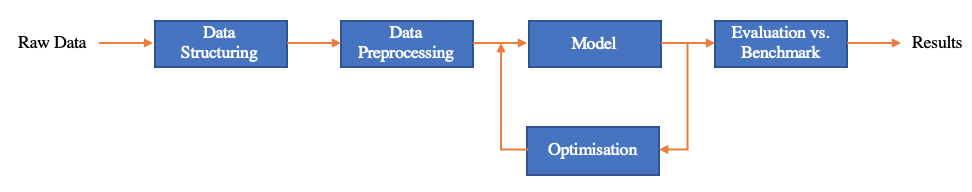
\includegraphics[width=14.5cm]{design_pipeline.png}
\caption{High-level overview of the tool pipeline design}
\label{pipeline_design}
\end{figure}

\subsection{Data Preprocessing}

\subsubsection{Overview}

Initially, sample formats were distributed in csv formats. However, when the entire dataset was actually provided, the file was stored in a .rds file because the firm mainly operated in R. It was then necessary to study the data storage structure in order to extract the relevant information that could be used for the project. 

The data is structured in lists of features. These are separated into 5 categories, two of which will be useful to this project. These will be \textit{Fundamentals} and \textit{Prices}. \textit{Fundamentals} is data about the company itself, such as book value or sales whereas \textit{Prices} is data regarding how the behavioural characteristics of the stock itself trades on the exchange. Each company is labelled with their unique ticker. Example: CNHI:IM which is the CNH Industrial NV. 

\textit{Fundamentals} is divided into two categories: Last Twelve Months (LTM) and Next Twelve Months (NTM). LTMs are the historical data points for the past year of a specific feature whereas NTMs are the predictions of those features for the next year. LTM contains 16 features and NTM contains 31 features. We are working with a subset of the Euro Stoxx 600 Index (SXXP) and so will only focus on companies that are categorised as Industrial Goods and Services. The Index ID for this is SXNP. There are 203 companies that fit this category. For each feature, there are 6313 data points, starting from 1995-01-03 (Y-D-M). 

\textit{Prices} is divided into two categories: Local and Euros which indicates the denomination that the values of the stocks are presented in. Because Local introduces an external factor of currency value fluctuation into the problem, it will be ignored and Euros will be used for its standardised format. Euros contains 14 features related to the technical indicators of the stock. Again, there are 203 companies for each of these features and the number of datapoints is 6313, starting from 1995-01-03 (Y-D-M). 

The other 3 categories are \textit{Mapping}, \textit{Signals} and \textit{Indices}. \textit{Mapping} provides the keys of the dataset and so can be used to select a specific subset that is of interest. This is what is used to filter out the original number of companies (1184) to the Industrials subset (203). \textit{Signals} provides 3 sets which looks at the investor sentiment. \textit{Indices} provides the pricing data of worldwide indices.  

\begin{figure}[!hbt!]
\centering
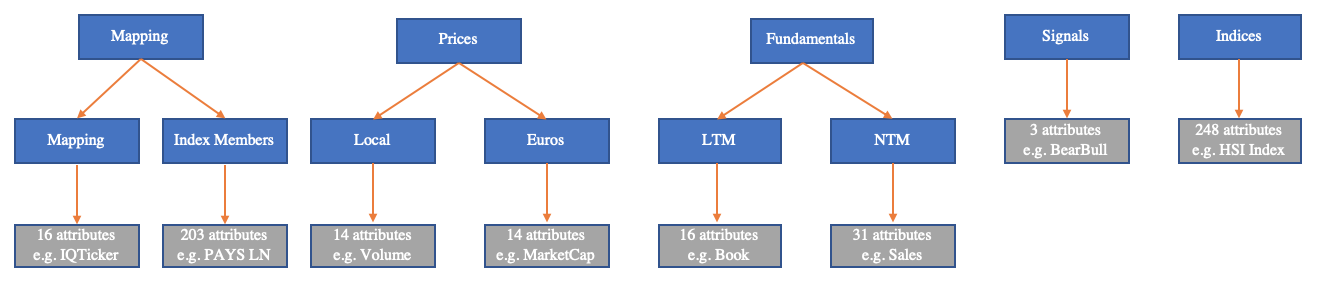
\includegraphics[width=14.5cm]{database.png}
\caption{Diagram overview of the database hierarchy.}
\end{figure}

\subsubsection{Handling Sparsity} \label{data_analysis}

\subsubsection{Data Transformation}

In order to have some directional predictive power, the delta of the attributes will be measured over rather than the absolute values i.e. $\frac{x_{t}}{x_{t+1}}$. This means that the underlying assumption is that the price of stock changes given changes in the \textit{Fundamentals} and \textit{Price} features. Unfortunately, given the sporadic nature of fundamental data reporting, which is often quarterly or longer, technical data is required to supplement the model. All missing data or deltas which are 0 will be masked and thus not affect the model. 


\subsection{Architectural Design} 

\subsubsection{Overview}

The design of the architecture was implemented in an iterative process, starting initially with the most basic baseline design consisting of one hidden layer. The idea was to evaluate the results of the designs and then modify or redesign them to improve the performance and accuracy. In order to identify the sets of models that could be used, the initial process involved identifying the inputs, outputs and target function that were suitable for the fundamental problem.

\subsubsection{Inputs}

The inputs for the model were initially intended be all of the usable features in the \textit{Fundamentals} category. This totalled approximately $15+16=32$. However, a section of the NTM category was labelled as original (e.g. EpsOriginal and Eps) and this was decided to be too raw a format for usage. It would also have caused duplications in the input vector, unintentionally giving some attributes double the weighting. At least one of the Price category attributes will be missing as it is the variable that needs to be predicted - namely the closing price.   

Although the project was initially intended to be based solely on analysing fundamental data, the lack of data reported as depicted in section \ref{data_analysis} resulted in concerns relating to the feasibility of learning in such a small dataset. This lack of data was attributed to the fact that values may not have been measured or recorded as much historically (1990s) and also that values are often only reported on a quarterly basis, resulting in only 4 data points each year compared to the 252 data points of the price. 

\subsubsection{Output}

\subsubsection{Loss Function}

\subsubsection{Design Interations}

\subsection{Benchmark Design} \label{benchmark}.

Our selected benchmark performance metric will be derived from the naive diversification choice heuristic. This means that for a given universe of $N$ stocks, a portfolio will be constructed by allocating a $\frac{1}{N}$ weighting to each stock. The interest here is in the efficiency of such a portfolio compared to those which are optimised to favour certain stocks achieved by overweighting them such that their allocations are greater than $\frac{1}{N}$. DeMiguel et al. conducted investigations\cite{DeMiguel} regarding 14 mean-variance optimisation models and found that there was no statistically significant improved performance relative to $\frac{1}{N}$ diversification. As such, it is of interest for investment managers to construct mathematical models that can outperform the simplistic model often utilised by less sophisticated investors for its ease-of-use. 

In order to evaluate this, the output values will be ordered and a theoretical portfolio constructed with respect to the percentage of the total sum of the outputs ($weighting(i) = \frac{output_{i} }{\sum_{i=1}^{N} output_{i}}$). It should be noted that the architecture of the network will be devised such that a larger output is better e.g. implies a higher return, lower volatility etc. Although this portfolio layout is by no means optimised for best performance, it succinctly describes and roughly equates to what stocks the model has selected to over and underweight. It is then possible to evaluate this portfolio with respect to three basic performance measure and compare and contrast to those of the naive diversification heuristic. 

\begin{itemize}
	\item Absolute Return: This is the most basic method of evaluation - observing how much return is generated by a portfolio over a given period of time. The simplicity of the measure allows it to be easily implemented and direct comparisons can be made between the model generated and benchmark figures. It is calculated by $100\times \frac{V_{end} - V_{start}}{V_{start}}$ where $V$ is the value of the portfolio and $start$ and $end$ are the beginning and finish times of the investment. A higher absolute return indicates better performance. 
	\item	Sharpe Ratio: First introduced by William Sharpe\cite{Sharpe} in 1966, this is a commonly used method of measuring risk adjusted return. Since a more risky investment should in theory offer a greater potential reward, a more insightful method of evaluation is judging whether the returns received are in line with the risk taken in a given portfolio. A simplified version will be used that does not account for the risk free rate to reduce complexity in calculations: $Simple Sharpe Ratio = \frac{R_{p}}{\sigma_{p}}$ where $R_{p}$ and $\sigma_p$ are the return and its standard deviation of the portfolio respectively. A higher Sharpe Ratio indicates better performance.  
	\item Portfolio Turnover: This measures how often the stocks within the portfolio have to be bought and sold to rebalance and maintain the model's strategy. Although it does not theoretically affect the performance, the transaction costs of buying and selling in a real world scenario can significantly affect a portfolio's profitability. Therefore a lower turnover is preferred. It is calculated with the following equation: $turnover = \frac{min(s_{b}, s_{s})}{NAV}$ where $NAV$ is the Net Asset Value and $s_{b}$ and $s_{s}$ are the cost of stocks bought and sold respectively.  
\end{itemize}

\subsection{Training and Testing} 

\subsection{Hyperparameter Optimisation} 

%-------------------------------------------------------------------------
\newpage

\section{Implementation}


Give code details - descriptions of key parts, annotated to help the reader understand what they are looking at. Good reasons for including code could be to illustrate algorithmic flow, or highlight an interesting optimisation, demonstrate interactions with a data-structure, or give an example of input for a tool that has been designed.

Discuss the most important or interesting aspects, and anything that was surprising or difficult. It probably won't be possible or relevant to discuss everything – state clearly what you leave out.

If you cannot explain what message or point a code fragment is conveying,  it probably should not be in the report, and if you cannot justify why a line of code in the fragment helps convey that point, it maybe it shouldn’t be in the code fragment.

For similar reasons, pasting screen-shots is unlikely to be a good use of space, unless it serves a particular purpose. Screen-shots are sometimes used instead of drawing a picture (for example as a “cheap” way of showing wave-forms or state machines), or in order to capture the results of running a tool (which will often be text anyway), and tend to look unprofessional and lazy. They are also sometimes used as page filler, or as “proof” that a tool was launched and something compiled, which is not necessary: your marker’s default position will be to believe your claims. Use a screen-shot if it is demonstrating a particular point, such as a failure mode in a tool, or a particular interaction that is difficult/impossible to highlight, but make sure you edit and annotate the figure to show and highlight the important parts.

When discussing the implementation, it is generally best to focus on the conceptual and logical design, and only then dive into details for interesting parts or to highlight important decisions. Well thought-out figures and diagrams are often much more effective at conveying your design than source code, whether that is a data-structure, a client-server interaction, a design-flow, or a circuit hierarchy. For example, a diagram of a block-diagram of digital circuit can be used to communicate to the reader most of the important high-level  decisions you have made, then VHDL fragments (or another diagram) could be used to focus on specific parts and demonstrate any interesting local details.

Complete listings may be included as appendices of your report but this is not normally appropriate, unless the appendix is documentation, or describes an API. Software may be provided on a CD-ROM given to your supervisor or in a cloud repositories such as Github. No marks are awarded for the mass or page count of a report, and reports which contain 50 pages of printed code are more likely to be seen as showing poor judgement

\subsection{Data structuring}
 
Given the large number of csv files, there was a necessity to store the resulting dataframes in a systematic method so that functions that needed to be performed on method could be done so efficiently. This was achieved by dividing the respective csv files first into input and traget variables. Of course, only one file was needed for the target variable, being the close price dataset. 

\begin{lstlisting}[language=Python, breaklines=true]
price_close = pd.read_csv('/content/drive/My Drive/thw116_FYP/data/price_close.csv')
\end{lstlisting}

However, given that there were much more input datasets, it was decided to store these dataframes in lists, based on the categories that they were originally allocated in the raw .rds file. 

\begin{lstlisting}[language=Python, breaklines=true]
ltm_book = pd.read_csv('/content/drive/My Drive/thw116_FYP/data/ltm_book.csv')
ltm_div = pd.read_csv('/content/drive/My Drive/thw116_FYP/data/ltm_div.csv')
........................
ltm_inputs = [ltm_book, ltm_div, ltm_ebit, ltm_ebitda, ltm_ebitda, ltm_eps, ltm_fcf, ltm_pbook, ltm_sales] 
ntm_inputs = [ntm_book, ntm_div, ntm_ebit, ntm_ebitda, ntm_ebitda, ntm_eps, ntm_fcf, ntm_pbook, ntm_sales]
tech_inputs = [price_high, price_low, price_open, volume, enterprise_val]
\end{lstlisting} 

This then made functions far easier to implement across all the data, such as in this instance where the dataframes were allocated a \textit{datetime} index. 

\begin{lstlisting}[language=Python, breaklines=true]
def time_index_generator(dataframe):
  dataframe['Date'] = pd.to_datetime(dataframe['Date'], dayfirst=True)
  dataframe.set_index('Date', inplace=True)

for i in range(0,len(ltm_inputs)):
  time_index_generator(ltm_inputs[i])
\end{lstlisting} 

After preprocessing across the dataset, it was necessary to reformat the data into an input form acceptable to the Keras model architecture. For this all of the lists of dataframes had to be iterated through and the appropriate datapoint extracted to create another list that would represent the input vector. 

\begin{lstlisting}[language=Python, breaklines=true]
trainInput = []
trainTarget = []

# Check that the indices are of the same length 
if len(ltm_trainInputs[0]) != len(returns_trainOutput):
  assert False, "Incompatible dataframe index lengths!"

for company in range(0, len(ltm_trainInputs[0][:1][0])):
  
  for time_unit in range(0, len(ltm_trainInputs[0])): 
    input_unit = []
    
    for ltm_attribute in range(0, len(ltm_trainInputs)): 
      input_unit.append(ltm_trainInputs[ltm_attribute][time_unit:time_unit+1][0][company])
                        
    for ntm_attribute in range(0, len(ntm_trainInputs)):
      input_unit.append(ntm_trainInputs[ntm_attribute][time_unit:time_unit+1][0][company])
                        
    for tech_attribute in range(0, len(tech_trainInputs)): 
      input_unit.append(tech_trainInputs[tech_attribute][time_unit:time_unit+1][0][company])
                        
    trainInput.append(input_unit)
    
for company in range(0, len(returns_trainOutput.columns)):
  for time_unit in range(0, len(returns_trainOutput.index)): 
    trainTarget.append(returns_trainOutput[anon_tickers[company]][time_unit])
\end{lstlisting} 

These lists were then converted into \textit{numpy} arrays. This provided the use of \textit{reshape} functionality only accessible to arrays as well as the fact that they are more memory and computationally efficient. Keras requires a Since this is the immediate step before inputting into the architecture, there is no more need for the flexibility offered by lists. 

\begin{lstlisting} 
trainInput, trainTarget = np.array(trainInput), np.array(trainTarget)
trainInput = np.reshape(trainInput, (trainInput.shape[0], trainInput.shape[1], 1))
\end{lstlisting} 





\subsection{Architecture} 

\begin{lstlisting}[language=Python, breaklines=true]
data_dim = trainInput.shape[1]
timesteps = trainInput.shape[0]

# Sample Code
# model parameters:

def create_model(train_X, train_Y, data_dim):
  lstm_units = 128
  
#   print('Build baseline binary model...')
#   model = Sequential()
#   model.add(Masking(mask_value=0., input_shape=(data_dim, 1)))
#   model.add(LSTM(lstm_units))
#   model.add(Dense(1))
#   model.compile(loss='binary_crossentropy', optimizer='adam', metrics=['accuracy'])
  
  
  print('Build stacked binary model')
  model = Sequential()
  model.add(Masking(mask_value=0., input_shape=(data_dim, 1)))
  model.add(LSTM(lstm_units, return_sequences=True))
  model.add(Dropout(0.2))
  model.add(LSTM(lstm_units, return_sequences=True))
  model.add(Dropout(0.2))

  model.add(LSTM(lstm_units))
  model.add(Dense(1))
  model.compile(loss='binary_crossentropy', optimizer='adam', metrics=['accuracy'])

  
  #   model.compile(loss='mean_squared_error', optimizer='adam', metrics=['accuracy'])

  return(model)

  
baseline_model = create_model(trainInput, trainTarget, data_dim)
SVG(model_to_dot(baseline_model, show_shapes=True).create(prog='dot', format='svg'))
\end{lstlisting} 


\subsection{Benchmark} 



%-------------------------------------------------------------------------
\newpage

\section{Testing}
Put the actual test results in an Appendix if they are repetitive but relevant. 
Detailed test data may be omitted from the report if not relevant, however an accurate summary of tests should be included in the Report itself. 
Sometimes non-working designs are described in project reports as though they work, when in reality they don’t, or only partially work. Therefore a precise description of what works and how this has been established is important. Examiners may try to compile, use, or test deliverables themselves (even after your report is submitted), and your report should accurately reflect
the state of the project.
This section is normally useful for software or hardware deliverables and less relevant in analytical projects.

\subsection{Test Plan} 

\begin{figure}[!hbt!]
\centering
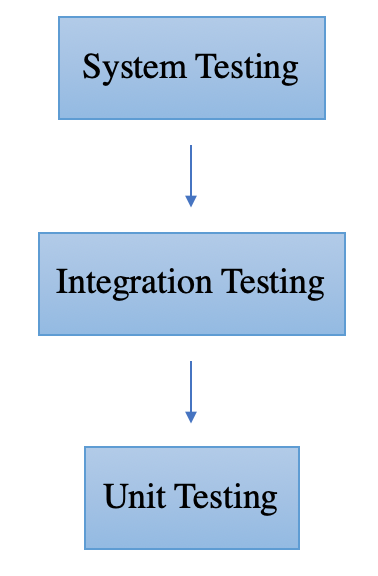
\includegraphics[width=3.5cm]{evaluation.png}
\caption{Levels of software testing from high (Top) to low (Bottom)}
\end{figure}

The procedure of evaluating the achievements of the project will vary according to the stage of the software development cycle. On the atomic level is the unit test, which will be used to validate that each of the separate modules and functions of the software are functioning as expected. An example\cite{python_testing} of how unit testing will be implemented is shown below. By using the assert statement in Python, it is possible to determine whether the function, $sum()$, is outputting the expected result of $6$. An incorrect result will raise an $AssertionError$ and output the message $not6$.

\begin{lstlisting}[language=Python]
def test_sum():
    assert sum([1, 2, 3]) == 6, "not6"
\end{lstlisting} 

The next level up involves integration testing, which focuses on the correctness of functionality in combined components of the software. An example of this would be examining the outputs of a function which takes as an input a processed dataframe from another function. It is important to test the combined behaviour of these two components after individual unit testing to ensure that it is in line with expectations. Given the data orientated nature of the project, this will mainly be achieved through the development of small, well-defined test datasets to compare and contrast with the outputs of the components.  

\begin{figure}[!hbt!]
\centering
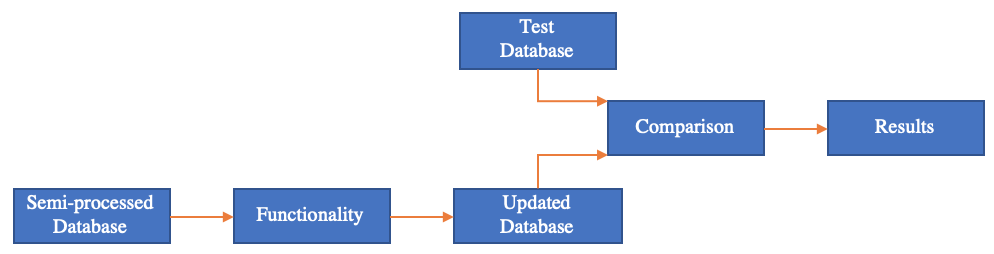
\includegraphics[width=15.5cm]{integrated_testing.png}
\caption{Flow diagram of how an integrated test may be executed.}
\end{figure}

System testing will involve evaluating the realised performance of the whole system. This will then allow for the model to be comparable to other methodologies developed in the field and industry.

\subsection{Test Results} 


%-------------------------------------------------------------------------
\newpage

\section{Results}

This covers an area different from the 'Testing'
chapter, and relates to the understanding and analysis
of the algorithm, program, or hardware behaviour.
Where the deliverable is a product with easily
quantified performance then the previous Chapter
shows how functional correctness is established,
while this Chapter shows qualitatively or
quantitatively how well the product works. The list
below shows typical content, not all of this will be
applicable to all projects.
An empirical relationship between
parameters and results may be investigated,
typically through the use of appropriate
graphs.
Where theory predicts aspects of
performance the results can be compared
with expectation and differences noted and (if
possible) explained.
Semi-empirical models of behaviour may be
developed, justified, and tested.
The types of experiments/simulations that
were carried out should be described. Why
were certain experiments carried out but not
others? What were the important parameters
in the simulation and how did they affect the
results? If there are very many graphs and
tables associated with this chapter they may
be put in the Appendix, but it is generally
better to keep these close to the text they
illustrate, as this is easier for the reader.

\subsection{Baseline}

%-------------------------------------------------------------------------
\newpage

\section{Evaluation}
This Chapter (or possibly section of the conclusions) is distinct from your results

critical evaluation of your work as compared to previous analysis, algorithms, products, and when related to your original objectives.
To what extent have your original objectives been fulfilled? 

If they have changed, what is your rationale for this? What are the advantages, disadvantages of your approach compared with related work? 

How does the scope of your work differ from related work? Examiners expect your project report to show evidence of your ability to think as an engineer, and that includes the ability to critically reflect on your own work and evaluate its significance. 

Material here will compare project outcomes with initial objectives and requirements captured. Usually your Interim Report will contain these. Where these have changed significantly over the course of the project this should be explained and reasons given. 

This section should not require examiners to read your Interim Report, and will not reference it. Changes between final and initial objectives should be explained in a self-contained manner. Note that here you will reference and summarise, rather than repeat, your description of Requirements Capture earlier in the Final Report.

%-------------------------------------------------------------------------
\newpage

\section{Conclusions}


How successful have you been? What have you achieved? How could the work be taken further given more time. It is important here to identify positively what is worthwhile in your work. At the same time, honesty, and a clear description of the limits of your work, is equally important. It is often most appropriate to describe work you did not have time to complete as further work.
Your readers will not be clear where, in your long report, are your most significant achievements. In the conclusions you must summarise this, referring as necessary to other sections for more detail.
What design choices did you have along the way, and why did you make the choices you made?
What was the most difficult and/or clever part of the project?
Why was it difficult? How did you overcome the difficulties?
Did you discover or invent anything novel?
What did you learn?
Note that “difficult” does not necessarily mean the thing that took you the longest amount of time. Note also that the conclusions must concisely summarise this material, and refer to other sections for the details.

\subsection{Future Work} 

\newpage

\section{Bibliography}

{
\small
\bibliographystyle{ieee}
\bibliography{thw116bib}
}

\newpage

\section{Appendix}
Please use appendices as necessary for material that is tangentially relevant, or necessary to preserve project value, but that you do not expect Examiners to read.

Related material possibly but not directly relevant to the project work. E.g. manuals of test equipment used. (There is no requirement to include such, but in some cases, where they have some tangential relevance, it might be appropriate).

\subsection{Source Code}
TC: The Appendix should normally include, or refer to, all the technical details needed for another user to continue code development.
Github repository

\subsection{Test data}
TC: The report itself will contain concise summaries of the test data in a human readable form.
Github repository

\end{document}
